\documentclass[10pt]{article}
\usepackage[a4paper,landscape,margin=9mm]{geometry}
\usepackage{amsmath,amssymb,newtxtext,newtxmath,graphicx,tikz,xcolor}
\usetikzlibrary{arrows.meta}
\usepackage[hidelinks]{hyperref}
\definecolor{ink}{HTML}{183D50}
\definecolor{paperblue}{HTML}{F2F6F8}
\pagestyle{empty}\setlength{\parindent}{0pt}
\newsavebox{\formulabox}
\newcommand{\fitmath}[1]{\sbox{\formulabox}{$#1$}\ifdim\wd\formulabox>\linewidth\resizebox{\linewidth}{!}{\usebox{\formulabox}}\else\usebox{\formulabox}\fi}
\begin{document}
{\color{ink}\fontsize{17}{21}\selectfont Theorem graph / 1. Existence, recovery, and the mean-value identity}\par\vspace{4pt}
{\small Arrows show dependencies within this panel. Other inputs are listed by ID on each card. Full records: \texttt{theorem\_graph/theorems.json}.}\par\vspace{6pt}
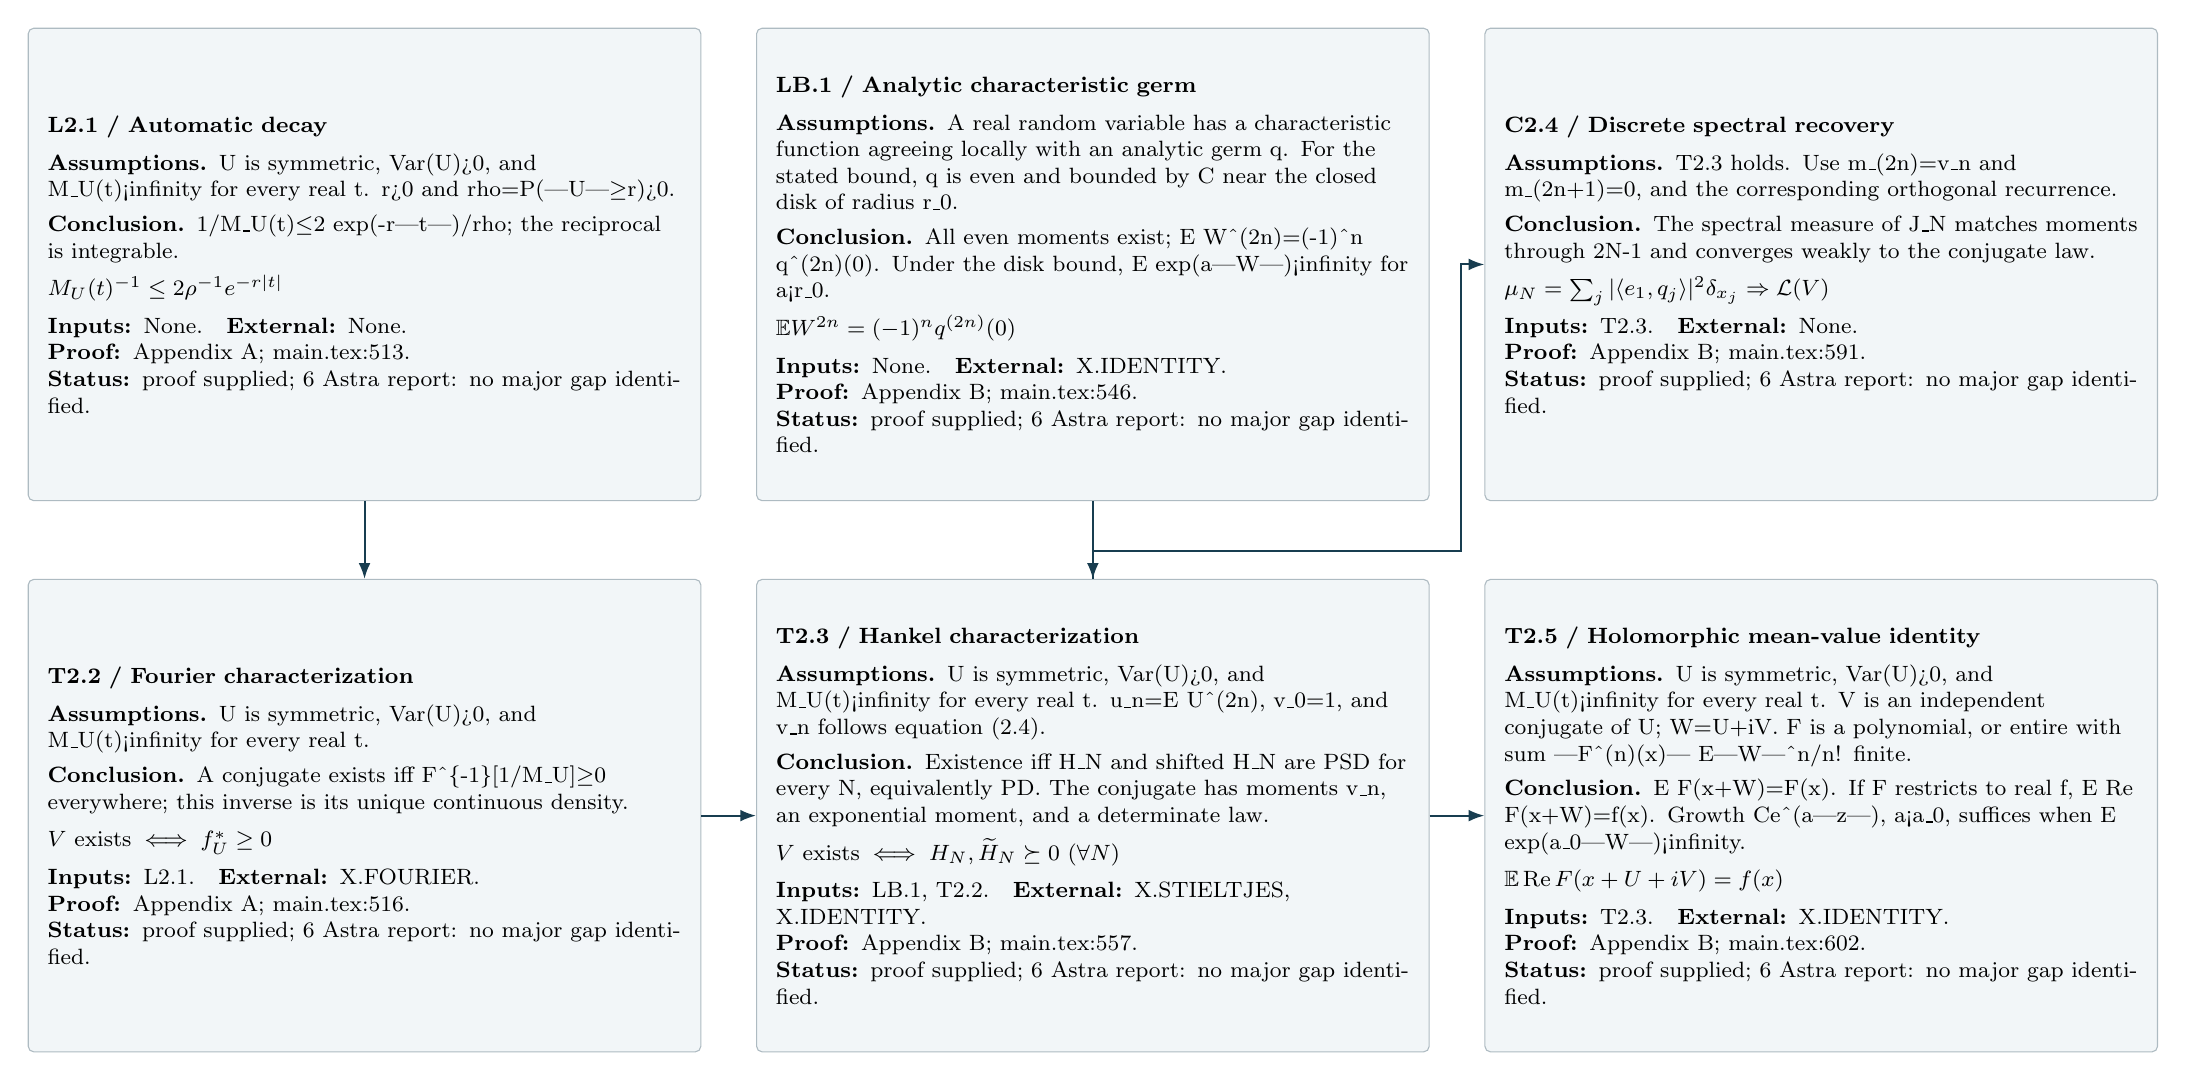
\begin{tikzpicture}[card/.style={draw=ink!35,fill=paperblue,rounded corners=2pt,anchor=north west,text width=8.05cm,inner sep=7pt,minimum height=6.0cm,align=left,font=\fontsize{8}{9.6}\selectfont\raggedright},dep/.style={-{Latex[length=2mm]},draw=ink,line width=.7pt}]
\node[card] (L21) at (0,0) {\raggedright\textbf{L2.1 / Automatic decay}\par\vspace{4pt}\textbf{Assumptions.} U is symmetric, Var(U)>0, and M\_U(t)<infinity for every real t. r>0 and rho=P(|U|$\ge$r)>0.\par\vspace{3pt}\textbf{Conclusion.} 1/M\_U(t)$\le$2 exp(-r|t|)/rho; the reciprocal is integrable.\par\vspace{4pt}\fitmath{M_U(t)^{-1}\le 2\rho^{-1}e^{-r|t|}}\par\vspace{4pt}\textbf{Inputs:} None.\quad\textbf{External:} None.\par\textbf{Proof:} Appendix A; main.tex:513.\par\textbf{Status:} proof supplied; 6 Astra report: no major gap identified.};
\node[card] (T22) at (0,-7) {\raggedright\textbf{T2.2 / Fourier characterization}\par\vspace{4pt}\textbf{Assumptions.} U is symmetric, Var(U)>0, and M\_U(t)<infinity for every real t.\par\vspace{3pt}\textbf{Conclusion.} A conjugate exists iff F\textasciicircum{}\{-1\}[1/M\_U]$\ge$0 everywhere; this inverse is its unique continuous density.\par\vspace{4pt}\fitmath{V\text{ exists}\iff f_U^*\ge0}\par\vspace{4pt}\textbf{Inputs:} L2.1.\quad\textbf{External:} X.FOURIER.\par\textbf{Proof:} Appendix A; main.tex:516.\par\textbf{Status:} proof supplied; 6 Astra report: no major gap identified.};
\node[card] (LB1) at (9.25,0) {\raggedright\textbf{LB.1 / Analytic characteristic germ}\par\vspace{4pt}\textbf{Assumptions.} A real random variable has a characteristic function agreeing locally with an analytic germ q. For the stated bound, q is even and bounded by C near the closed disk of radius r\_0.\par\vspace{3pt}\textbf{Conclusion.} All even moments exist; E W\textasciicircum{}(2n)=(-1)\textasciicircum{}n q\textasciicircum{}(2n)(0). Under the disk bound, E exp(a|W|)<infinity for a<r\_0.\par\vspace{4pt}\fitmath{\mathbb E W^{2n}=(-1)^nq^{(2n)}(0)}\par\vspace{4pt}\textbf{Inputs:} None.\quad\textbf{External:} X.IDENTITY.\par\textbf{Proof:} Appendix B; main.tex:546.\par\textbf{Status:} proof supplied; 6 Astra report: no major gap identified.};
\node[card] (T23) at (9.25,-7) {\raggedright\textbf{T2.3 / Hankel characterization}\par\vspace{4pt}\textbf{Assumptions.} U is symmetric, Var(U)>0, and M\_U(t)<infinity for every real t. u\_n=E U\textasciicircum{}(2n), v\_0=1, and v\_n follows equation (2.4).\par\vspace{3pt}\textbf{Conclusion.} Existence iff H\_N and shifted H\_N are PSD for every N, equivalently PD. The conjugate has moments v\_n, an exponential moment, and a determinate law.\par\vspace{4pt}\fitmath{V\text{ exists}\iff H_N,\widetilde H_N\succeq0\ (\forall N)}\par\vspace{4pt}\textbf{Inputs:} LB.1, T2.2.\quad\textbf{External:} X.STIELTJES, X.IDENTITY.\par\textbf{Proof:} Appendix B; main.tex:557.\par\textbf{Status:} proof supplied; 6 Astra report: no major gap identified.};
\node[card] (C24) at (18.5,0) {\raggedright\textbf{C2.4 / Discrete spectral recovery}\par\vspace{4pt}\textbf{Assumptions.} T2.3 holds. Use m\_(2n)=v\_n and m\_(2n+1)=0, and the corresponding orthogonal recurrence.\par\vspace{3pt}\textbf{Conclusion.} The spectral measure of J\_N matches moments through 2N-1 and converges weakly to the conjugate law.\par\vspace{4pt}\fitmath{\mu_N=\sum_j|\langle e_1,q_j\rangle|^2\delta_{x_j}\Rightarrow\mathcal L(V)}\par\vspace{4pt}\textbf{Inputs:} T2.3.\quad\textbf{External:} None.\par\textbf{Proof:} Appendix B; main.tex:591.\par\textbf{Status:} proof supplied; 6 Astra report: no major gap identified.};
\node[card] (T25) at (18.5,-7) {\raggedright\textbf{T2.5 / Holomorphic mean-value identity}\par\vspace{4pt}\textbf{Assumptions.} U is symmetric, Var(U)>0, and M\_U(t)<infinity for every real t. V is an independent conjugate of U; W=U+iV. F is a polynomial, or entire with sum |F\textasciicircum{}(n)(x)| E|W|\textasciicircum{}n/n! finite.\par\vspace{3pt}\textbf{Conclusion.} E F(x+W)=F(x). If F restricts to real f, E Re F(x+W)=f(x). Growth Ce\textasciicircum{}(a|z|), a<a\_0, suffices when E exp(a\_0|W|)<infinity.\par\vspace{4pt}\fitmath{\mathbb E\operatorname{Re}F(x+U+iV)=f(x)}\par\vspace{4pt}\textbf{Inputs:} T2.3.\quad\textbf{External:} X.IDENTITY.\par\textbf{Proof:} Appendix B; main.tex:602.\par\textbf{Status:} proof supplied; 6 Astra report: no major gap identified.};
\draw[dep] (L21.south) -- (T22.north);
\draw[dep] (LB1.south) -- (T23.north);
\draw[dep] (T22.east) -- (T23.west);
\draw[dep] (T23.north) -- ++(0,0.35) -| ([xshift=-0.3cm]C24.west) -- (C24.west);
\draw[dep] (T23.east) -- (T25.west);
\end{tikzpicture}\par\vspace{3pt}
{\fontsize{8}{10}\selectfont\textbf{External dependency status.} X.FOURIER: classical; applied and detailed in Appendix A. X.IDENTITY: classical; applied with explicit domains. X.STIELTJES: classical; cited, not reproved.}
\newpage
{\color{ink}\fontsize{17}{21}\selectfont Theorem graph / 2. Polynomial realization}\par\vspace{4pt}
{\small Arrows show dependencies within this panel. Other inputs are listed by ID on each card. Full records: \texttt{theorem\_graph/theorems.json}.}\par\vspace{6pt}
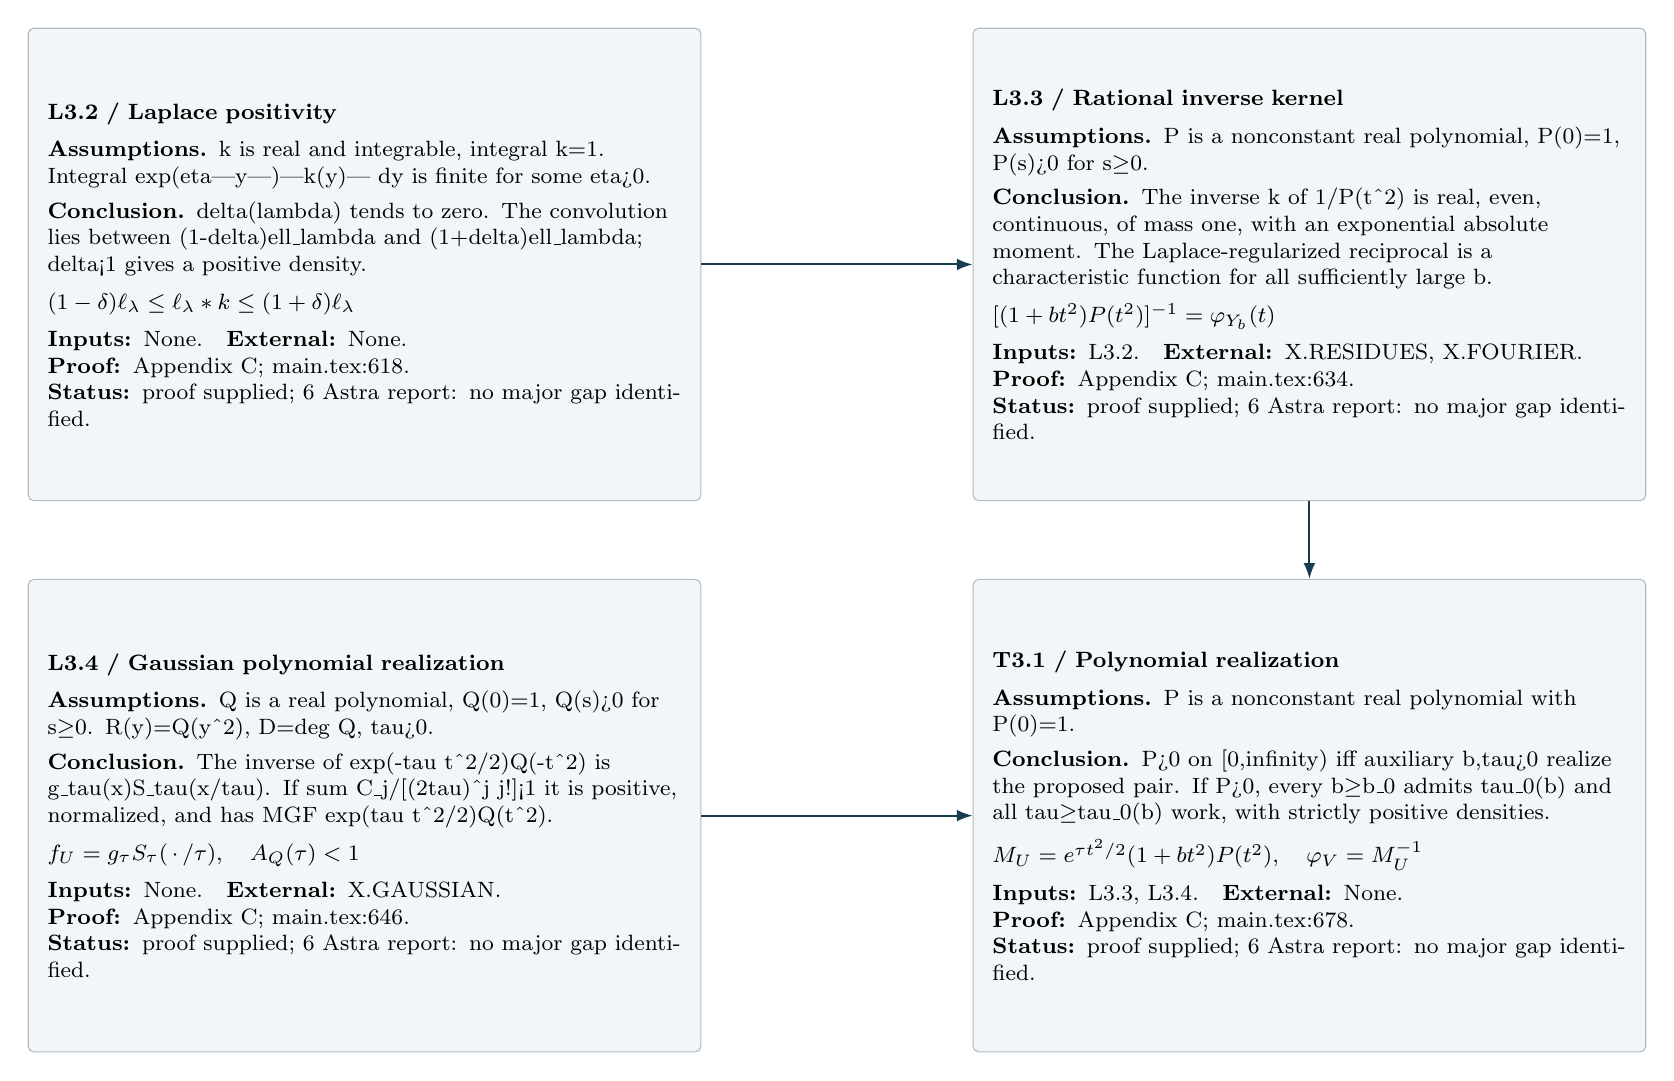
\begin{tikzpicture}[card/.style={draw=ink!35,fill=paperblue,rounded corners=2pt,anchor=north west,text width=8.05cm,inner sep=7pt,minimum height=6.0cm,align=left,font=\fontsize{8}{9.6}\selectfont\raggedright},dep/.style={-{Latex[length=2mm]},draw=ink,line width=.7pt}]
\node[card] (L32) at (3,0) {\raggedright\textbf{L3.2 / Laplace positivity}\par\vspace{4pt}\textbf{Assumptions.} k is real and integrable, integral k=1. Integral exp(eta|y|)|k(y)| dy is finite for some eta>0.\par\vspace{3pt}\textbf{Conclusion.} delta(lambda) tends to zero. The convolution lies between (1-delta)ell\_lambda and (1+delta)ell\_lambda; delta<1 gives a positive density.\par\vspace{4pt}\fitmath{(1-\delta)\ell_\lambda\le\ell_\lambda*k\le(1+\delta)\ell_\lambda}\par\vspace{4pt}\textbf{Inputs:} None.\quad\textbf{External:} None.\par\textbf{Proof:} Appendix C; main.tex:618.\par\textbf{Status:} proof supplied; 6 Astra report: no major gap identified.};
\node[card] (L33) at (15,0) {\raggedright\textbf{L3.3 / Rational inverse kernel}\par\vspace{4pt}\textbf{Assumptions.} P is a nonconstant real polynomial, P(0)=1, P(s)>0 for s$\ge$0.\par\vspace{3pt}\textbf{Conclusion.} The inverse k of 1/P(t\textasciicircum{}2) is real, even, continuous, of mass one, with an exponential absolute moment. The Laplace-regularized reciprocal is a characteristic function for all sufficiently large b.\par\vspace{4pt}\fitmath{[(1+bt^2)P(t^2)]^{-1}=\varphi_{Y_b}(t)}\par\vspace{4pt}\textbf{Inputs:} L3.2.\quad\textbf{External:} X.RESIDUES, X.FOURIER.\par\textbf{Proof:} Appendix C; main.tex:634.\par\textbf{Status:} proof supplied; 6 Astra report: no major gap identified.};
\node[card] (L34) at (3,-7) {\raggedright\textbf{L3.4 / Gaussian polynomial realization}\par\vspace{4pt}\textbf{Assumptions.} Q is a real polynomial, Q(0)=1, Q(s)>0 for s$\ge$0. R(y)=Q(y\textasciicircum{}2), D=deg Q, tau>0.\par\vspace{3pt}\textbf{Conclusion.} The inverse of exp(-tau t\textasciicircum{}2/2)Q(-t\textasciicircum{}2) is g\_tau(x)S\_tau(x/tau). If sum C\_j/[(2tau)\textasciicircum{}j j!]<1 it is positive, normalized, and has MGF exp(tau t\textasciicircum{}2/2)Q(t\textasciicircum{}2).\par\vspace{4pt}\fitmath{f_U=g_\tau S_\tau(\,\cdot\,/\tau),\quad A_Q(\tau)<1}\par\vspace{4pt}\textbf{Inputs:} None.\quad\textbf{External:} X.GAUSSIAN.\par\textbf{Proof:} Appendix C; main.tex:646.\par\textbf{Status:} proof supplied; 6 Astra report: no major gap identified.};
\node[card] (T31) at (15,-7) {\raggedright\textbf{T3.1 / Polynomial realization}\par\vspace{4pt}\textbf{Assumptions.} P is a nonconstant real polynomial with P(0)=1.\par\vspace{3pt}\textbf{Conclusion.} P>0 on [0,infinity) iff auxiliary b,tau>0 realize the proposed pair. If P>0, every b$\ge$b\_0 admits tau\_0(b) and all tau$\ge$tau\_0(b) work, with strictly positive densities.\par\vspace{4pt}\fitmath{M_U=e^{\tau t^2/2}(1+bt^2)P(t^2),\quad \varphi_V=M_U^{-1}}\par\vspace{4pt}\textbf{Inputs:} L3.3, L3.4.\quad\textbf{External:} None.\par\textbf{Proof:} Appendix C; main.tex:678.\par\textbf{Status:} proof supplied; 6 Astra report: no major gap identified.};
\draw[dep] (L32.east) -- (L33.west);
\draw[dep] (L33.south) -- (T31.north);
\draw[dep] (L34.east) -- (T31.west);
\end{tikzpicture}\par\vspace{3pt}
{\fontsize{8}{10}\selectfont\textbf{External dependency status.} X.FOURIER: classical; applied and detailed in Appendix A. X.GAUSSIAN: classical; derivative formula derived in Appendix C. X.RESIDUES: classical; contour argument given in Appendix C.}
\newpage
{\color{ink}\fontsize{17}{21}\selectfont Theorem graph / 3. Structural exclusions and the explicit family}\par\vspace{4pt}
{\small Arrows show dependencies within this panel. Other inputs are listed by ID on each card. Full records: \texttt{theorem\_graph/theorems.json}.}\par\vspace{6pt}
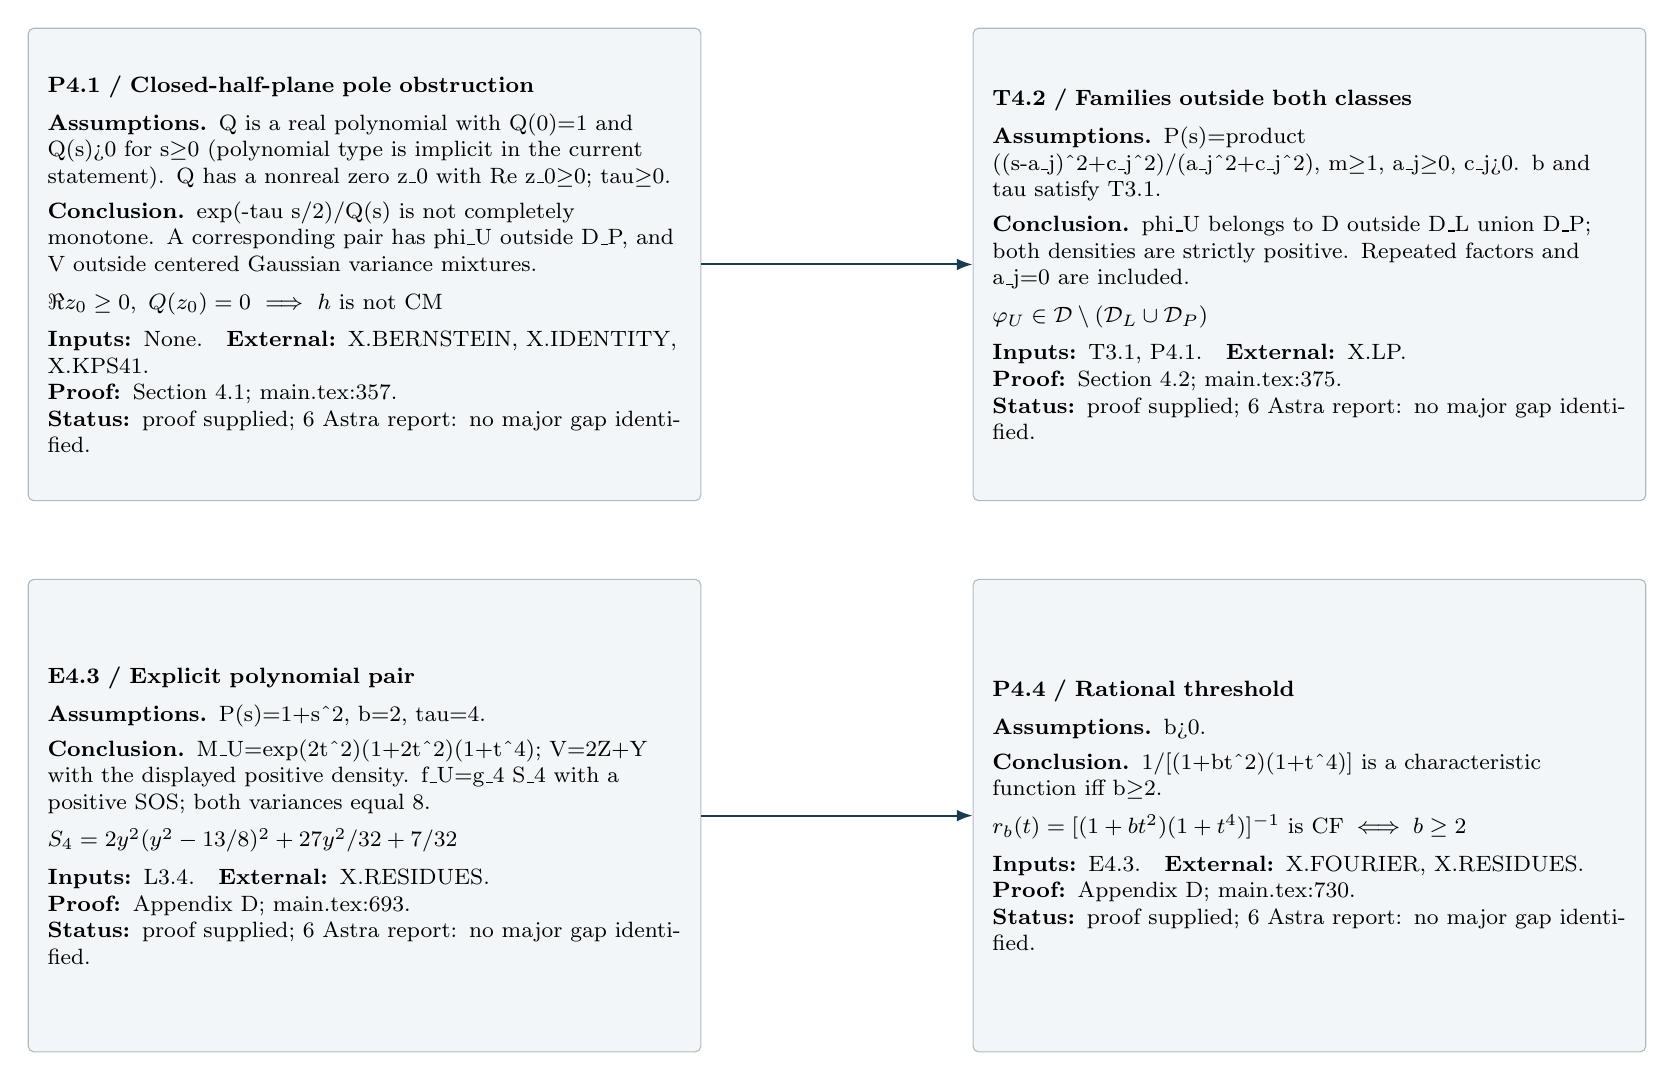
\begin{tikzpicture}[card/.style={draw=ink!35,fill=paperblue,rounded corners=2pt,anchor=north west,text width=8.05cm,inner sep=7pt,minimum height=6.0cm,align=left,font=\fontsize{8}{9.6}\selectfont\raggedright},dep/.style={-{Latex[length=2mm]},draw=ink,line width=.7pt}]
\node[card] (P41) at (3,0) {\raggedright\textbf{P4.1 / Closed-half-plane pole obstruction}\par\vspace{4pt}\textbf{Assumptions.} Q is a real polynomial with Q(0)=1 and Q(s)>0 for s$\ge$0 (polynomial type is implicit in the current statement). Q has a nonreal zero z\_0 with Re z\_0$\ge$0; tau$\ge$0.\par\vspace{3pt}\textbf{Conclusion.} exp(-tau s/2)/Q(s) is not completely monotone. A corresponding pair has phi\_U outside D\_P, and V outside centered Gaussian variance mixtures.\par\vspace{4pt}\fitmath{\Re z_0\ge0,\ Q(z_0)=0\ \Longrightarrow\ h\text{ is not CM}}\par\vspace{4pt}\textbf{Inputs:} None.\quad\textbf{External:} X.BERNSTEIN, X.IDENTITY, X.KPS41.\par\textbf{Proof:} Section 4.1; main.tex:357.\par\textbf{Status:} proof supplied; 6 Astra report: no major gap identified.};
\node[card] (T42) at (15,0) {\raggedright\textbf{T4.2 / Families outside both classes}\par\vspace{4pt}\textbf{Assumptions.} P(s)=product ((s-a\_j)\textasciicircum{}2+c\_j\textasciicircum{}2)/(a\_j\textasciicircum{}2+c\_j\textasciicircum{}2), m$\ge$1, a\_j$\ge$0, c\_j>0. b and tau satisfy T3.1.\par\vspace{3pt}\textbf{Conclusion.} phi\_U belongs to D outside D\_L union D\_P; both densities are strictly positive. Repeated factors and a\_j=0 are included.\par\vspace{4pt}\fitmath{\varphi_U\in\mathcal D\setminus(\mathcal D_L\cup\mathcal D_P)}\par\vspace{4pt}\textbf{Inputs:} T3.1, P4.1.\quad\textbf{External:} X.LP.\par\textbf{Proof:} Section 4.2; main.tex:375.\par\textbf{Status:} proof supplied; 6 Astra report: no major gap identified.};
\node[card] (E43) at (3,-7) {\raggedright\textbf{E4.3 / Explicit polynomial pair}\par\vspace{4pt}\textbf{Assumptions.} P(s)=1+s\textasciicircum{}2, b=2, tau=4.\par\vspace{3pt}\textbf{Conclusion.} M\_U=exp(2t\textasciicircum{}2)(1+2t\textasciicircum{}2)(1+t\textasciicircum{}4); V=2Z+Y with the displayed positive density. f\_U=g\_4 S\_4 with a positive SOS; both variances equal 8.\par\vspace{4pt}\fitmath{S_4=2y^2(y^2-13/8)^2+27y^2/32+7/32}\par\vspace{4pt}\textbf{Inputs:} L3.4.\quad\textbf{External:} X.RESIDUES.\par\textbf{Proof:} Appendix D; main.tex:693.\par\textbf{Status:} proof supplied; 6 Astra report: no major gap identified.};
\node[card] (P44) at (15,-7) {\raggedright\textbf{P4.4 / Rational threshold}\par\vspace{4pt}\textbf{Assumptions.} b>0.\par\vspace{3pt}\textbf{Conclusion.} 1/[(1+bt\textasciicircum{}2)(1+t\textasciicircum{}4)] is a characteristic function iff b$\ge$2.\par\vspace{4pt}\fitmath{r_b(t)=[(1+bt^2)(1+t^4)]^{-1}\text{ is CF}\iff b\ge2}\par\vspace{4pt}\textbf{Inputs:} E4.3.\quad\textbf{External:} X.FOURIER, X.RESIDUES.\par\textbf{Proof:} Appendix D; main.tex:730.\par\textbf{Status:} proof supplied; 6 Astra report: no major gap identified.};
\draw[dep] (P41.east) -- (T42.west);
\draw[dep] (E43.east) -- (P44.west);
\end{tikzpicture}\par\vspace{3pt}
{\fontsize{8}{10}\selectfont\textbf{External dependency status.} X.BERNSTEIN: classical; cited, not reproved. X.FOURIER: classical; applied and detailed in Appendix A. X.IDENTITY: classical; applied with explicit domains. X.KPS41: primary statement checked; used as an external theorem. X.LP: classical representation used to identify the comparison class. X.RESIDUES: classical; contour argument given in Appendix C.}
\newpage
{\color{ink}\fontsize{17}{21}\selectfont Theorem graph / 4. Recovery of known classes}\par\vspace{4pt}
{\small Arrows show dependencies within this panel. Other inputs are listed by ID on each card. Full records: \texttt{theorem\_graph/theorems.json}.}\par\vspace{6pt}
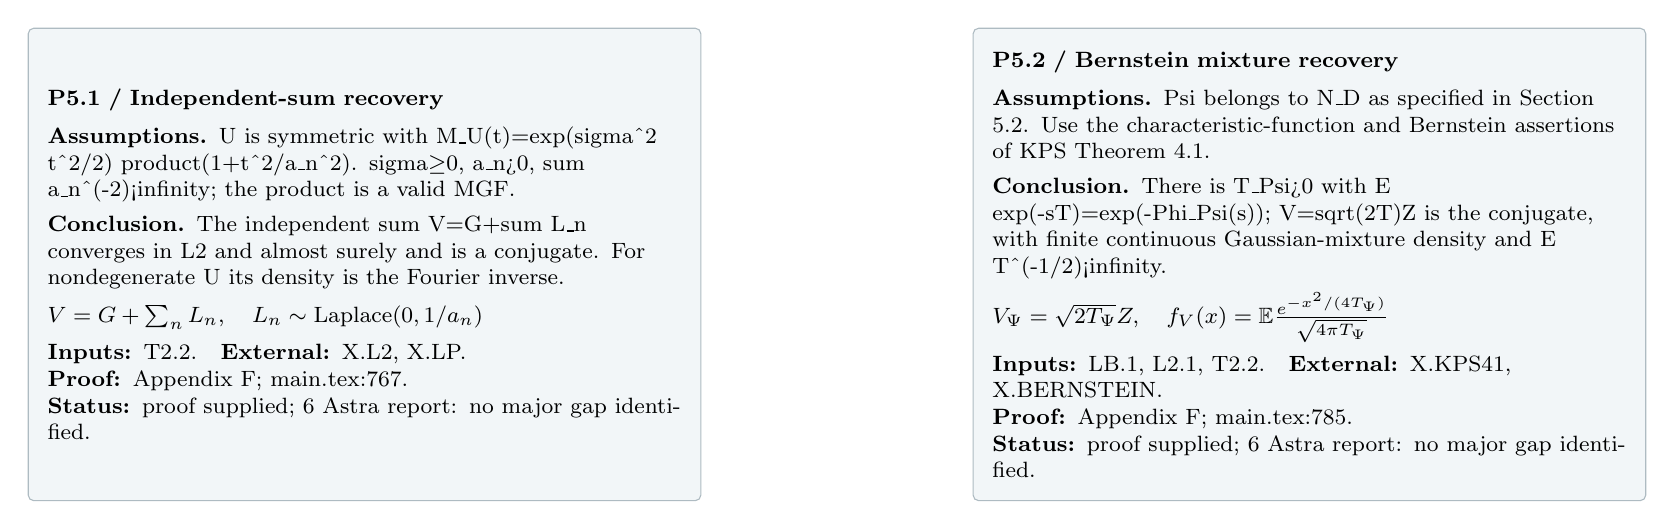
\begin{tikzpicture}[card/.style={draw=ink!35,fill=paperblue,rounded corners=2pt,anchor=north west,text width=8.05cm,inner sep=7pt,minimum height=6.0cm,align=left,font=\fontsize{8}{9.6}\selectfont\raggedright},dep/.style={-{Latex[length=2mm]},draw=ink,line width=.7pt}]
\node[card] (P51) at (3,0) {\raggedright\textbf{P5.1 / Independent-sum recovery}\par\vspace{4pt}\textbf{Assumptions.} U is symmetric with M\_U(t)=exp(sigma\textasciicircum{}2 t\textasciicircum{}2/2) product(1+t\textasciicircum{}2/a\_n\textasciicircum{}2). sigma$\ge$0, a\_n>0, sum a\_n\textasciicircum{}(-2)<infinity; the product is a valid MGF.\par\vspace{3pt}\textbf{Conclusion.} The independent sum V=G+sum L\_n converges in L2 and almost surely and is a conjugate. For nondegenerate U its density is the Fourier inverse.\par\vspace{4pt}\fitmath{V=G+\sum_n L_n,\quad L_n\sim\operatorname{Laplace}(0,1/a_n)}\par\vspace{4pt}\textbf{Inputs:} T2.2.\quad\textbf{External:} X.L2, X.LP.\par\textbf{Proof:} Appendix F; main.tex:767.\par\textbf{Status:} proof supplied; 6 Astra report: no major gap identified.};
\node[card] (P52) at (15,0) {\raggedright\textbf{P5.2 / Bernstein mixture recovery}\par\vspace{4pt}\textbf{Assumptions.} Psi belongs to N\_D as specified in Section 5.2. Use the characteristic-function and Bernstein assertions of KPS Theorem 4.1.\par\vspace{3pt}\textbf{Conclusion.} There is T\_Psi>0 with E exp(-sT)=exp(-Phi\_Psi(s)); V=sqrt(2T)Z is the conjugate, with finite continuous Gaussian-mixture density and E T\textasciicircum{}(-1/2)<infinity.\par\vspace{4pt}\fitmath{V_\Psi=\sqrt{2T_\Psi}Z,\quad f_V(x)=\mathbb E\frac{e^{-x^2/(4T_\Psi)}}{\sqrt{4\pi T_\Psi}}}\par\vspace{4pt}\textbf{Inputs:} LB.1, L2.1, T2.2.\quad\textbf{External:} X.KPS41, X.BERNSTEIN.\par\textbf{Proof:} Appendix F; main.tex:785.\par\textbf{Status:} proof supplied; 6 Astra report: no major gap identified.};
\end{tikzpicture}\par\vspace{3pt}
{\fontsize{8}{10}\selectfont\textbf{External dependency status.} X.BERNSTEIN: classical; cited, not reproved. X.KPS41: primary statement checked; used as an external theorem. X.L2: classical; applied in Appendix F. X.LP: classical representation used to identify the comparison class.}
\par\vspace{10pt}{\small\textbf{Reading the registry.} Every result has a stable ID, hypotheses, conclusion, proof and statement locations, internal dependencies, external dependency status, and contribution role. Source hashes bind the graph to the manuscript version.\par\vspace{5pt}X.KPS41 supplies the Bernstein representation for $\mathcal D_P$. X.LP supplies the classical product representation for class identification; P5.1 assumes that the displayed product is a valid moment-generating function.\par\vspace{5pt}\textbf{Review status.} The user-supplied 6 Astra report identifies no major mathematical gap. The two recorded editorial clarifications and the outstanding historical comparison are retained in the JSON.}
\end{document}
